% Note to reader: lines beginning with the '%' character are
% 'comments' to you, the human reader of this code, and are 
% ignored by the LaTeX compiler.

%%%%%%%%%%%%%%%%%%%%%%%%%%%%%%%%%%%%%%%%%%%%%%%%%%%%%%%%%%%%%%%%%%
% = Sample template for MIT Junior Lab Student Written Summaries =
% Available from 
%    http://web.mit.edu/8.13/www/Samplepaper/sample-paper.tex
%
% Last Updated July 23, 2014
%
% Adapted from the American Physical Societies REVTeK-4.1 Pages
%    at http://publish.aps.org
%
% ADVICE TO STUDENTS: Each time you write a paper, start with this
%    template and save under a new filename.  If convenient, don't
%    erase unneeded lines, just comment them out using the 
%    '%' character at the start of the line.  Often, they
%    will be useful containers for information.
%
% Using pdflatex, images must be either PNG, GIF, JPEG or PDF.
%    Turn EPS (encapsulated postscript) images to PDF using the
%    epstopdf utility on UNIX systems.
%%%%%%%%%%%%%%%%%%%%%%%%%%%%%%%%%%%%%%%%%%%%%%%%%%%%%%%%%%%%%%%%%%

%%%%%%%%%%%%%%%%%%%%%%%%%%%%%%%%%%%%%%%%%%%%%%%%%%%%%%%%%%%%%%%%%%
% = TO COMPILE THIS DOCUMENT =
%
% From the command line, it would go like this --- assuming you are
%    in the directory where the filename.tex source file and the 
%    filename.bib bibliography file are located, and that you have 
%    permission to create and write files in that directory:
%      > pdflatex filename
%      > bibtex filename
%      > pdflatex filname
%      > pdflatex filename
%    Yes, you run the command several times. The earlier runs 
%    create auxilliary files which keep track of references,
%    citations, equation and section numberring, etc. The later
%    runs combine the information in these auxilliary files with
%    your source document to create the finished product.
%
% If you are using a GUI LaTeX editor like TeXWorks, then there
%    is probably a menu bar button for pdfLaTeX and another for
%    BibTeX. Hit them in the order indicated above. There is 
%    probably also a 'TeXify' button, or something similarly named,
%    which runs all the above commands in one shot.     
%%%%%%%%%%%%%%%%%%%%%%%%%%%%%%%%%%%%%%%%%%%%%%%%%%%%%%%%%%%%%%%%%%


%%%%%%%%%%%%%%%%%%%%%%%%%%%%%%%%%%%%%%%%%%%%%%%%%%%%%%%%%%%%%%%%%%
%  = PREAMBLE =
% The preamble of a LaTeX document is the set of commands that precede
% the \begin{document} line.  It contains a \documentclass line
% to load the REVTeK-4.1 macro definitions and various \usepackage
% lines to load other macro packages.
%
% ADVICE TO STUDENTS: This preamble contains a suggested set of
%     class options to generate a ``Junior Lab'' look and feel that
%     facilitate quick review and feedback from one's peers, TAs,
%     and section instructors.  Don't make substantial changes 
%     to the style without first consulting your section 
%     instructor.
%%%%%%%%%%%%%%%%%%%%%%%%%%%%%%%%%%%%%%%%%%%%%%%%%%%%%%%%%%%%%%%%%%

%\documentclass[aps,twocolumn,secnumarabic,balancelastpage,amsmath,amssymb,nofootinbib, floatfix]{revtex4}
\documentclass[aps,twocolumn,nobalancelastpage,secnumarabic,amsmath,amssymb,nofootinbib,floatfix]{revtex4-1}

%%%%%%%%%%%%%%%%%%%%%%%%%%%%%%%%%%%%%%%%%%%%%%%%%%%%%%%%%%%%%%%%%%%
% N.B.:  Different computers have different packages installed.  
%        To compile this template in the current Athena 
%        environment, REVTeX 4.1 must be used.  To use the older
%        REVTeX 4, switch which documentclass line above is 
%        commented out above. There are ``bad'' distributions of
%        LaTeX for Windows available on the internet which may 
%        cause users to struggle unjustifiably with REVTeX 4.1.
%
%        If you are unable to compile the template at all, you
%        may need to update your LaTeX packages. (Alternatively, if 
%        your LaTeX distribution includes only the older RevTEX 4,
%        then try changing the documentclass line above. In particular,
%        this approach solves a common compilation problem for users of
%        the TeXWorks editor on Windows, which presents erroneously as a
%        error in the bibliography file.) Don't hesitate to speak 
%        with your section instructor or a TA if you're having 
%        issues getting this template to compile.
%%%%%%%%%%%%%%%%%%%%%%%%%%%%%%%%%%%%%%%%%%%%%%%%%%%%%%%%%%%%%%%%%%%

%%%%%%%%%%%%%%%%%%%%%%%%%%%%%%%%%%%%%%%%%%%%%%%%%%%%%%%%%%%%%%%%%%%
% = Explanation of documentclass options =
%
% aps, prl stand for American Physical Society and Physical 
%     Review Letters respectively.
% twocolumn permits two columns, of course.
% nobalancelastpage doesn't attempt to equalize the lengths of 
%     the two columns on the last page  as might be desired in a 
%     journal where articles follow one another closely.
% amsmath and amssymb are necessary for the subequations 
%     environment among others. These functionalities can
%     also be added use the usepackage function described below,
%     but REVTeX conveniently includes them as documentclass
%     options.
% secnumarabic identifies sections by number to aid electronic 
%     review and commentary.
% nofootinbib forces footnotes to occur on the page where they are
%      first referenced and not in the bibliography.
% floatfix attempts to help LaTeX decide where to place ``floats'',
%      like figures and plots, when it gets stuck and can't decide
%      by it's normal algorithm.
% REVTeX 4.1 is a set of macro packages designed to be used with 
%      LaTeX 2e. REVTeX is well-suited for preparing manuscripts 
%      for submission to APS journals.
%
% = Other documentclasses =
%
% The 'revtex4' and 'revtex4-1' documentclasses are somewhat 
%    specialized for making documents in the style of the APS
%    journals. For a more standard or generic looking LaTeX paper,
%    you could try any of the built-in documentclasses, in 
%    particular 'article' or 'report'. Someday, you may try to use 
%    the 'mitthesis'  documentclass available for download from the 
%    MIT Libraries. The vast majority of source code written for 
%    one documentclass should work just fine in any other, but 
%    occasional quirks arise. For example, some documentclasses 
%    disagree on whether the abstract declaration should come 
%    before or after the \begin{document} declaration.
% 
%%%%%%%%%%%%%%%%%%%%%%%%%%%%%%%%%%%%%%%%%%%%%%%%%%%%%%%%%%%%%%%%%%%

%% Now, include some packages which provide new commands that 
%% extend LaTeX's capabilities. Note that the nearly-essential
%% AMS math packages were added already as documentclass options
%% for REVTeX, but could have been added here using 
%% \usepackage{amsmath}, etc. The pacakges below are commonly 
%% useful, but there are many, many more available to solve a 
%% multitude of typesetting quandries (google your problem), 
%% and you  probably have the necesary packages installed on your
%% system already. Among the examples listed below, this sample
%% document only actually makes use of the 'graphicx', 'bm', 
%% and 'hyperref' pacakges, so the others are commented out for
%% tidyness.


\usepackage{graphicx}      % tools for importing graphics
\usepackage{lipsum}
\usepackage{float}
%\usepackage{lgrind}        % convert program code listings to a form 
                            % includable in a LaTeX document
%\usepackage{xcolor}        % produces boxes or entire pages with 
                            % colored backgrounds
%\usepackage{longtable}     % helps with long table options
%\usepackage{epsf}          % old package handles encapsulated postscript issues
\usepackage{bm}            % special bold-math package. usge: \bm{mathsymbol}
\usepackage{physics}
\usepackage{tensor}
%\usepackage{asymptote}     % For typesetting of mathematical illustrations
%\usepackage{thumbpdf}
\usepackage[colorlinks=true]{hyperref}  % this package should be added after 
                                        % all others.
                                        % usage: \url{http://web.mit.edu/8.13}


%%%%%%%%%%%%%%%%%%%%%%%%%%%%%%%%%%%%%%%%%%%%%%%%%%%%%%%%%%%%%%%%%%%
% And now, begin the document...
%%%%%%%%%%%%%%%%%%%%%%%%%%%%%%%%%%%%%%%%%%%%%%%%%%%%%%%%%%%%%%%%%%%

\begin{document}
\title{Relativistic Dynamic Detection through Electron Acceleration}
\author{Henry Shackleton}
\email{hshackle@mit.edu}
\date{\today}
\affiliation{MIT Department of Physics}


\begin{abstract}
  Classical and relativsitic mechanics differ in their predictions of how the momentum and energy of particles depend on their velocity. By accelerating electrons emitted from a $\tensor*[^{90}]{\text{Sr}}{}$ source through a magnetic field, we are able to measure these momentum and energy relations for the electrons. Using this, we are able to conclude that the relativistic theory more accurately predicts the trends measured. Fitting this relation also allows us to calculate the elctron charge to mass ratio, $e/m$.
\end{abstract}

\maketitle
\section{Introduction}
Albert Einstein's 1905 paper, "On the Electrodynamics of Moving Bodies," was one of the foundational papers to developing the theory of special relativity. This theory was intended to reconcile inconsistencies with classical mechanics, electrodynamics, and observed phenomena. In his paper, Einstein postulated that the speed of light is a constant value in all reference frames, contradicting the classical prediction that light travels faster or slower depending on one's speed relaive to the light. This postulate, along with the additional assumption that the laws of physics are the same in all reference frames, leads to a new theory of dynamics, with different predictions than classical mechanics. These discrepencies allow us to compare the two theories against experimental data, and thus determine which theory yields more accurate predictions. We test this theory by accelerating electrons to speeds close to the speed of light - the regime where classical and relativistic theories differ the most.

In classical mechanics, the kinetic energy $K$ of a particle as a function of momentum $p$ is given by
\begin{equation}
  K = \frac{p^2}{2m}
\end{equation}
where $m$ is the mass of the particle. Most notably, the kinetic energy as a function of momentum is quadratic.

In special relativity, the kinetic energy of a particle as a function of momentum is instead given by
\begin{equation}
  K = \sqrt{p^2 c^2 + m^2c^4} - mc^2
\end{equation}
where $c$ is the speed of light - approximately $3.0 \times 10^{8}$ km/s. The value $mc^2$ is known as the \textit{rest energy} of a particle. For particles with a small rest energy, $K$ becomes approximately a linear function of $p$. For massless particles like photons, $K(p)$ is exactly linear. 

These predictions from classical mechanics and special relativity gives us relations that can be used to fit an experimentally-measured graph of $K(p)$. The remainder of our analysis of the physical theory will be used to dermine how the kinetic energy and momentum of a particle relate to our setup.

The Lorentz law is an equation that holds in both classical mechanics and special relativity. This law determines how electric and magnetic fields affect the motion of a charged particle. In the presence of an electric field $\vb{E}$ and a magnetic field $\vb{B}$, the change in momentum is related to the two fields, as well as the charge of the particle $e$, the velocity of the particle $\vb{v}$, and the speed of light $c$ by
\begin{equation}
    \dv{\vb{p}}{t} = e\left(\vb{E} + \frac{\vb{v}}{c} \times \vb{B} \right)
  \end{equation}
  Equation $(3)$ implies that charged particles subject to a constant magnetic field will move in orbits in the plane perpendicular to the magnetic field, with a radius of rotation proportional to the momentum of the particle. Specifically, a particle subject to a constant magnetic field of magnitude $B$ that has a radius of rotation $\rho$ will have momentum 
  \begin{equation}
    p = \left(\frac{e\rho}{c}\right) B
  \end{equation}

\section{Experimental Setup}
Our experimental setup consists of a large, spherical shell with coils wrapped around it. When these coils are fed a current, it generates an approximately uniform magnetic field across the inside of the shell, oriented vertically. By varying the current supplied to the coils, we can control the magnetic field inside the shell. The top and bottom hemispheres of the shell are disconnected, to allow for inspection of the internal components of the shell.

In the bottom hemisphere of the shell, a vacuum chamber is maintained through a mechanical pump and monitored by a pressure gauge. On one side of the chamber, a $\tensor*[^{90}]{\text{Sr}}{}$/$\tensor*[^{90}]{\text{Y}}{}$ beta source is placed. This beta source emits electrons with energies up to $2.28$ MeV. When electrons are emitted in the prsence of the magnetic field, their trajectories are curved into orbits relative to their momentum.

On the other side of the chamber, placed at a distance of $40.6 \pm 0.4$ cm away from the source, is a parallel-plate velocity selector and a PIN diode detector. When the electrons are accelerated in a helical orbit, only electrons of a certain momentum will pass between the two plates. If these electrons continue on their helical orbit, they will hit the side of the plates and not be detected by the PIN diode. By supplying a constant electric field $E$ between the two plates , the trajectory of the elctrons can be straightened out and detected by the PIN diode at some $E$ proportional to the velocity of the electrons. When the electrons come in contact with the PIN diode, the kinetic energy is converted into an electric signal, which is fed through an amplifier and read by a multi-channel analyzer (MCA). This configuration allows us to detect the velocity, momentum, and kinetic energy of incoming electrons by looking at the supplied electric field, magnetic field, and MCA readout respectively.

Located halfway between the helical trajectory between the beta source and the detector is a metal divider with a small slit in it. In the absence of a perfect vacuum, our vacuum chamber will be filled with other particles, which the electrons from our beta source can scatter off of. To minimize the effects of this, we place a slit to attempt to screen our particles and only allow particles to pass through the slit whose trajectories have not been altered by scattering.

\begin{figure}[h]
  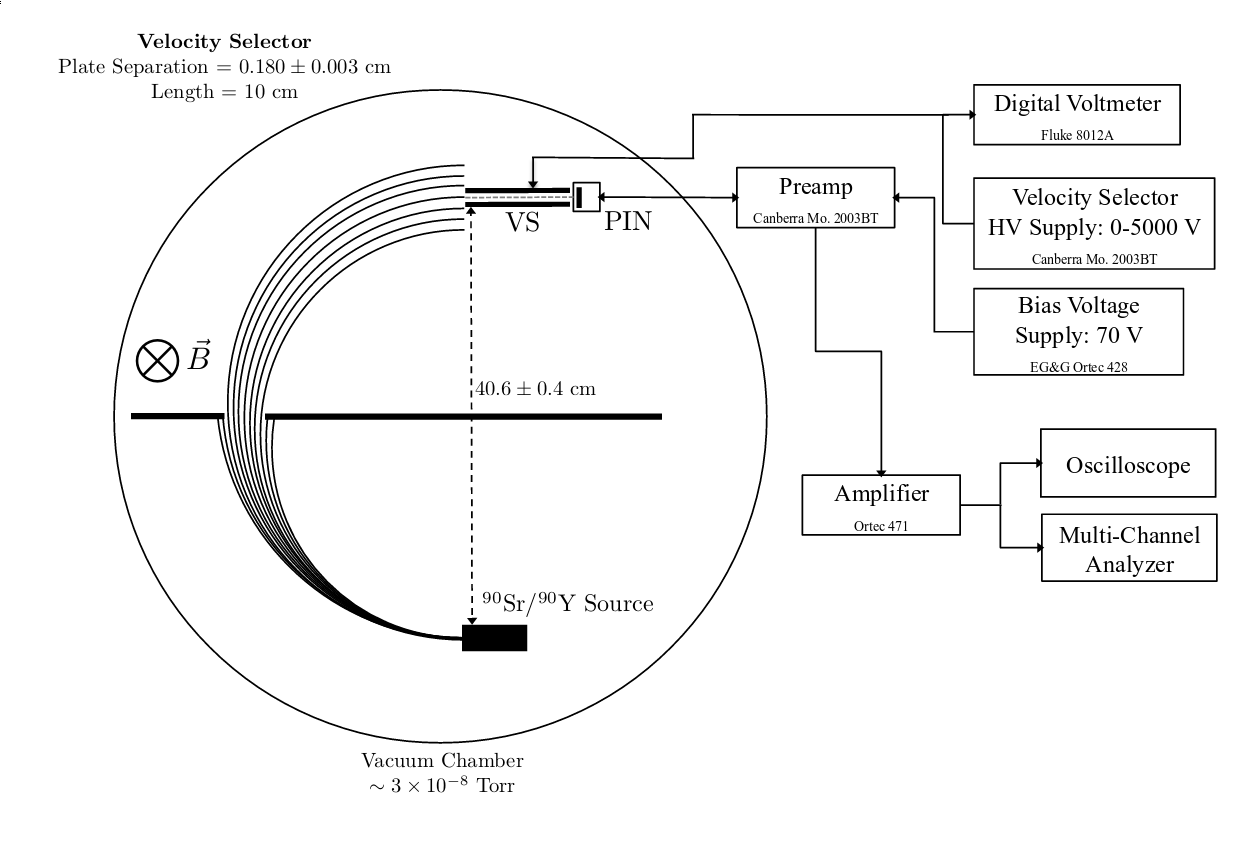
\includegraphics[width=.5\textwidth]{setup.png}
  \caption{A block diagram of our experimental setup. The circular lines drawn depict the expected trajectories from the beta source to the PIN diode detector.}
\end{figure}

\section{Experimental Calibration}
There are two calibration procedures necessary for this experiment - the MCA calibration and the magnetometer calibration. The MCA detects the strength of incoming electric signals and bins them accordingly, but the correspondance between this measurement and the kinetic energy of the detected electron is, by default, unknown. To determine this relation, we place a $\tensor*[^133]{\text{Ba}}{}$ source next to the PIN diode. The spectrum of $\tensor*[^133]{\text{Ba}}{}$ is well known and can be used to calibrate our MCA. Displayed in Figure $2$ is an example of an MCA readout of a $\tensor*[^133]{\text{Ba}}{}$ source, with various peaks labeled. In Table $1$, the energy known to correspond to these peaks is listed. Using this data, we can calibrate our MCA to display the kinetic energy of incoming electrons. 

To measure the magnetic field supplied to our electrons, we use a Hall effect magnetometer. 




%%%%%%%%%%%%%%%%%%%%%%%%%%%%%%%%%%%%%%%%%%%%%%%%%%%%%%%%%%%%%%%%%%


\end{document}
